\section{Giao diện đăng nhập}

Giao diện đăng nhập cho phép người dùng nhập thông tin xác thực và truy cập hệ thống
theo quyền được cấp.

\begin{figure}[H]
    \centering
    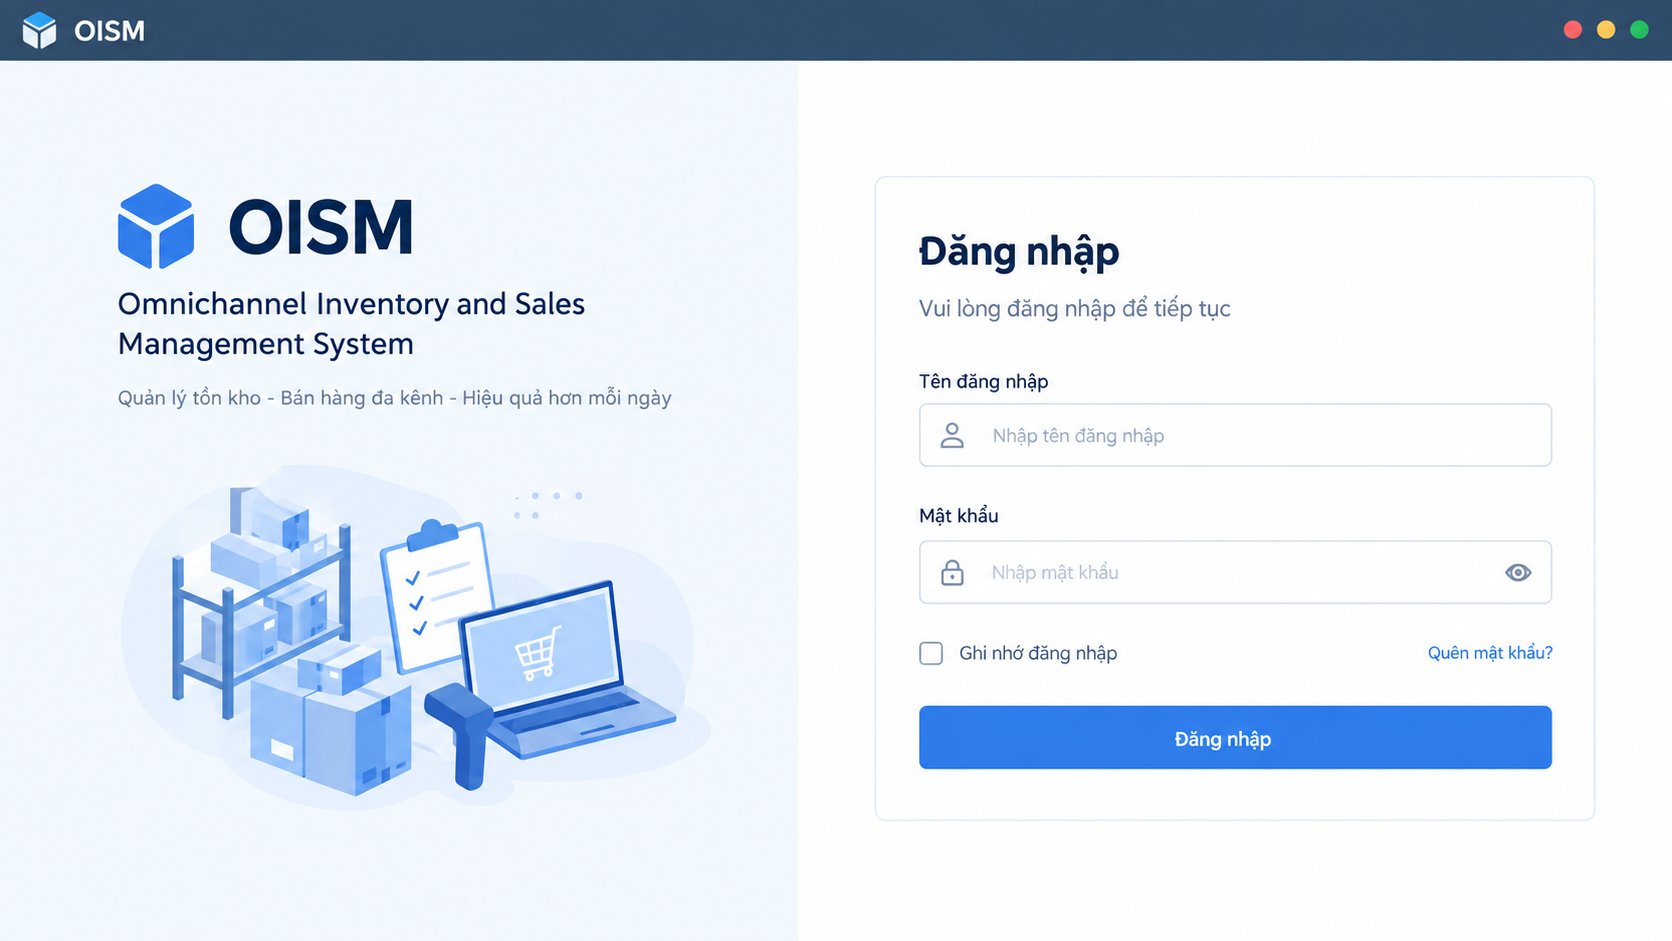
\includegraphics[
        width=0.92\textwidth,
        keepaspectratio
    ]{figures/dangnhap.png}
    \caption{Giao diện đăng nhập}
    \label{fig:ui-login}
\end{figure}

\section{Giao diện quản lý sản phẩm}

Màn hình quản lý sản phẩm hỗ trợ theo dõi danh mục, thương hiệu, biến thể, SKU,
mã vạch và thông tin giá bán.

\begin{figure}[H]
    \centering
    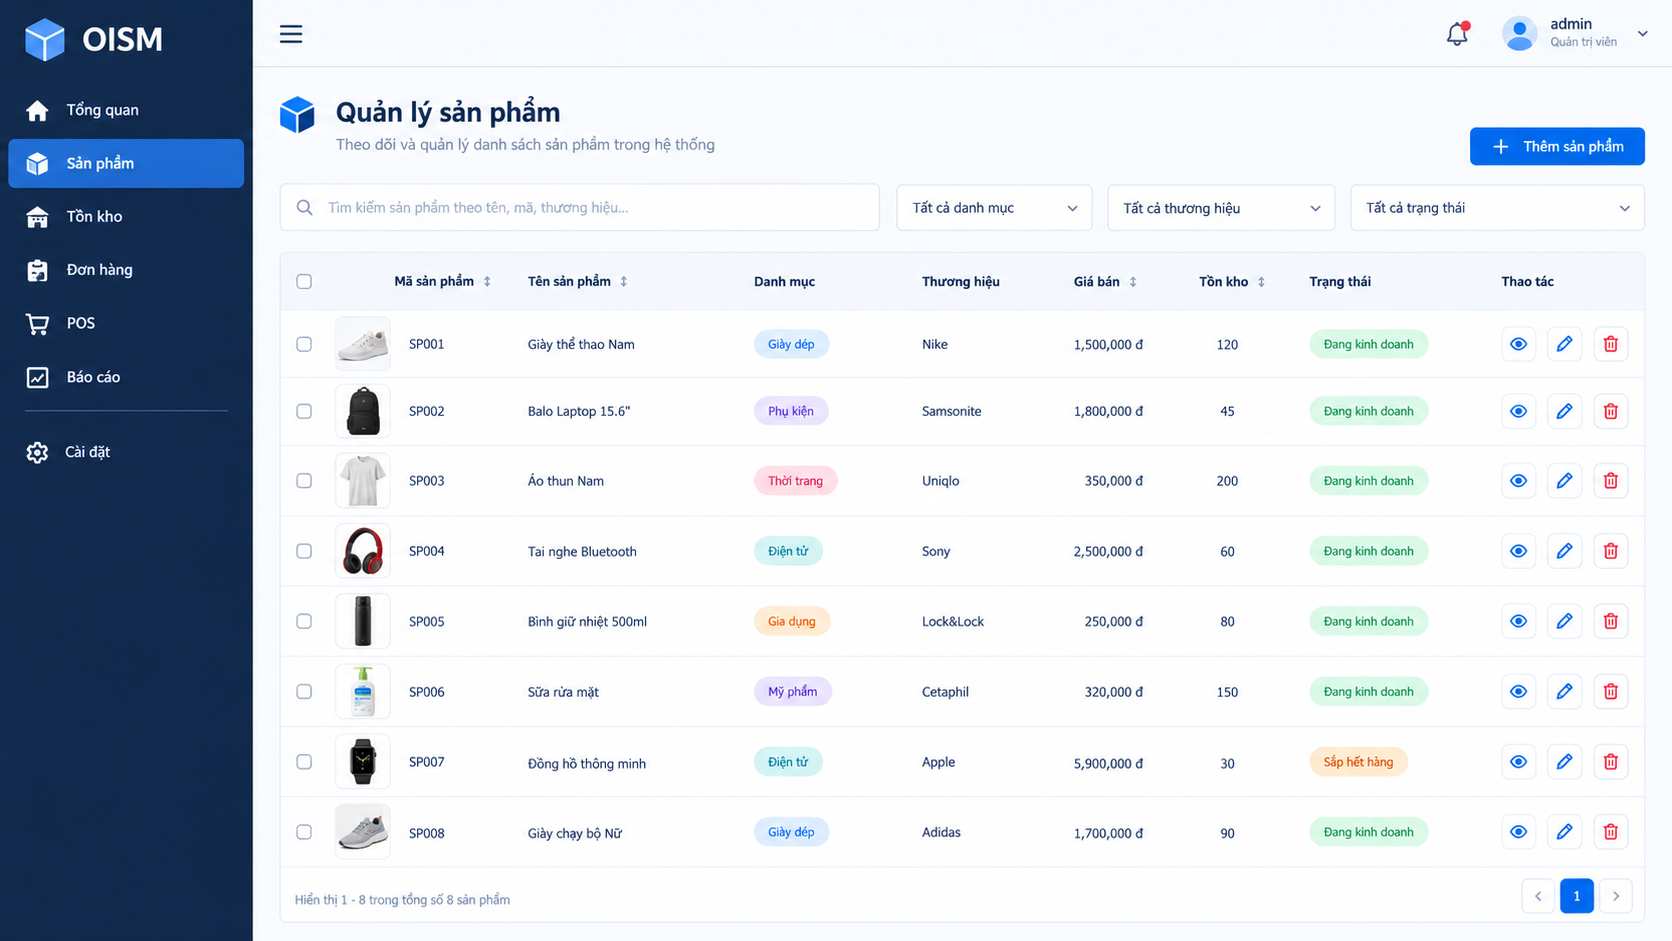
\includegraphics[
        width=0.92\textwidth,
        keepaspectratio
    ]{figures/quanly.png}
    \caption{Giao diện quản lý sản phẩm}
    \label{fig:ui-product}
\end{figure}

\section{Giao diện quản lý tồn kho}

Màn hình quản lý tồn kho cho phép theo dõi số lượng hàng hóa, các biến động nhập xuất
và trạng thái tồn kho theo chi nhánh.

\begin{figure}[H]
    \centering
    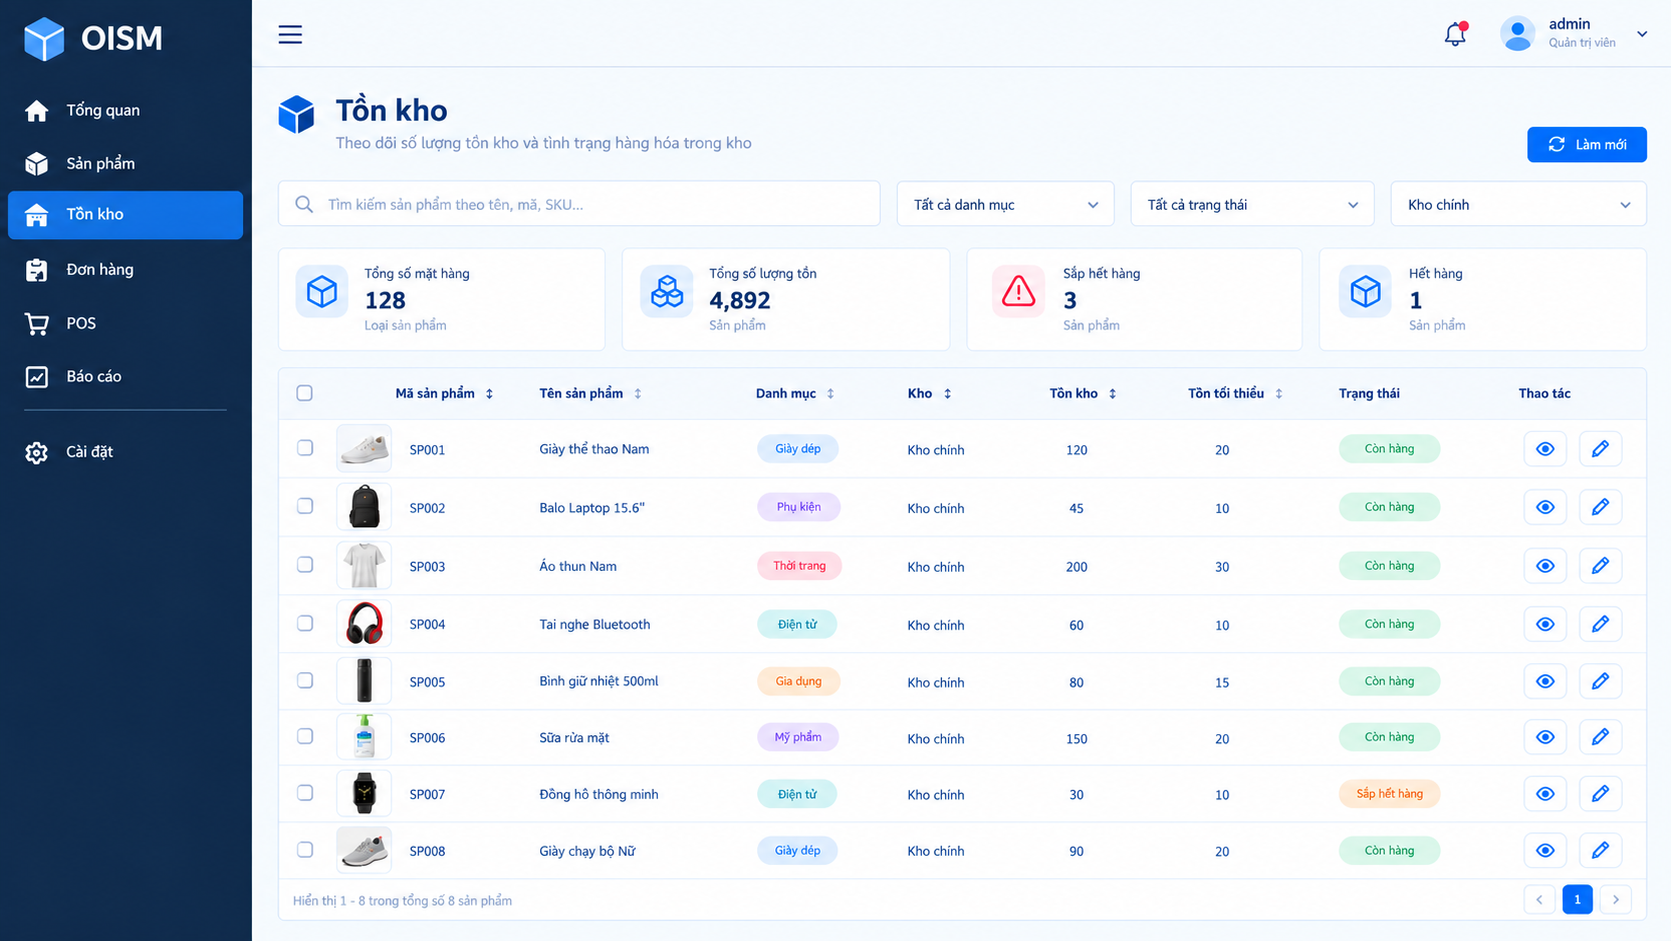
\includegraphics[
        width=0.92\textwidth,
        keepaspectratio
    ]{figures/tonkho.png}
    \caption{Giao diện quản lý tồn kho}
    \label{fig:ui-inventory}
\end{figure}

\section{Giao diện quản lý đơn hàng}

Màn hình đơn hàng tập trung hiển thị các đơn hàng từ nhiều kênh bán hàng và trạng thái
xử lý của từng đơn.

\begin{figure}[H]
    \centering
    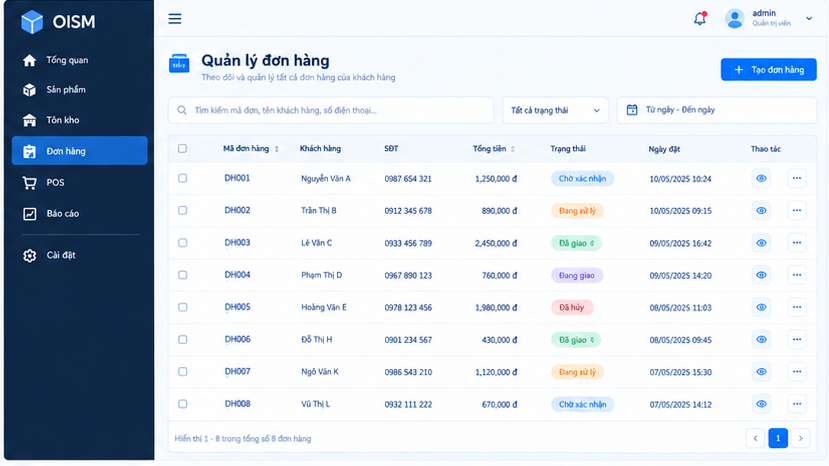
\includegraphics[
        width=0.92\textwidth,
        keepaspectratio
    ]{figures/donhang.png}
    \caption{Giao diện quản lý đơn hàng}
    \label{fig:ui-order}
\end{figure}

\section{Giao diện POS}

Giao diện POS được thiết kế ưu tiên thao tác nhanh, tìm kiếm sản phẩm và kiểm tra tồn kho
trước khi hoàn tất giao dịch.

\begin{figure}[H]
    \centering
    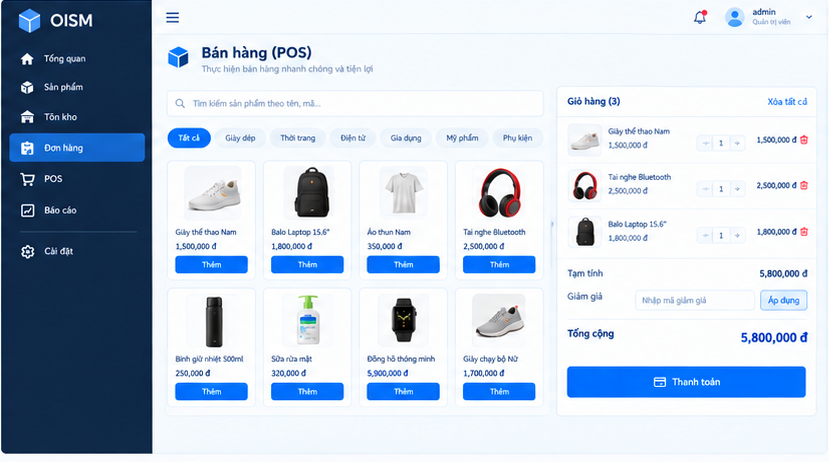
\includegraphics[
        width=0.92\textwidth,
        keepaspectratio
    ]{figures/POSs.png}
    \caption{Giao diện bán hàng tại POS}
    \label{fig:ui-pos}
\end{figure}

\section{Giao diện báo cáo}

Màn hình báo cáo trình bày các thông tin tổng quan về doanh thu, lợi nhuận gộp,
tình hình tồn kho và các cảnh báo liên quan.

\begin{figure}[H]
    \centering
    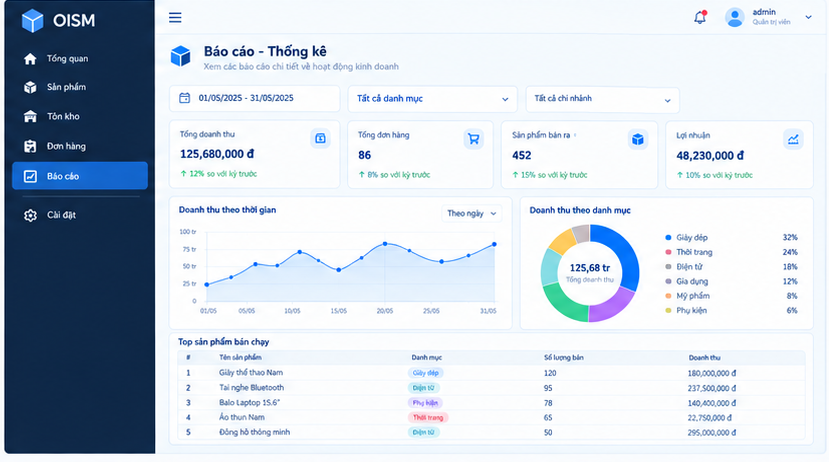
\includegraphics[
        width=0.92\textwidth,
        keepaspectratio
    ]{figures/baocao.png}
    \caption{Giao diện báo cáo}
    \label{fig:ui-report}
\end{figure}

\section{Nhận xét về giao diện}

Các giao diện được tổ chức theo nhóm chức năng, giúp người dùng dễ tìm kiếm thông tin
và thực hiện các nghiệp vụ chính. Khi hoàn thiện, nhóm có thể bổ sung ảnh chụp màn hình
thực tế vào các vị trí giữ chỗ ở trên.
